\section{Ergebnisse}

% Visualisierung
% reflectivity
% Vertikalgeschwindigkeit
% Hagel

Zunächst werden die Simulationen mithilfe von \textit{ParaView} visualisiert, dies dient dazu, einen Überblick über die komplexen Strukturen der Superzellen zu gewinnen und stellt sicher, dass die Ergebnisse plausibel sind und es keinen Fehler im Simulationsprozess gab. Beispielhaft wird ein Frame der Visualisierung in \cref{fig:singleframe} präsentiert, die kompletten Videos aller Simulationen sind über diesen \href{https://poincare.met.fu-berlin.de/~rw0064fu/cm1-anim/}{Link}\footnote{\hypersetup{urlcolor=}\url{https://poincare.met.fu-berlin.de/~rw0064fu/cm1-anim/}} abrufbar. Da Simulationsdaten nur alle \SI{5}{\min} zur Verfügung stehen, wird ein \textit{temporal interpolator} verwendet, allerdings sind weiterhin unschöne Sprünge zwischen den Frames erkennbar und die zeitliche Auflösung hätte weiter künstlich erhöht werden können.

\begin{figure}
	\centering
	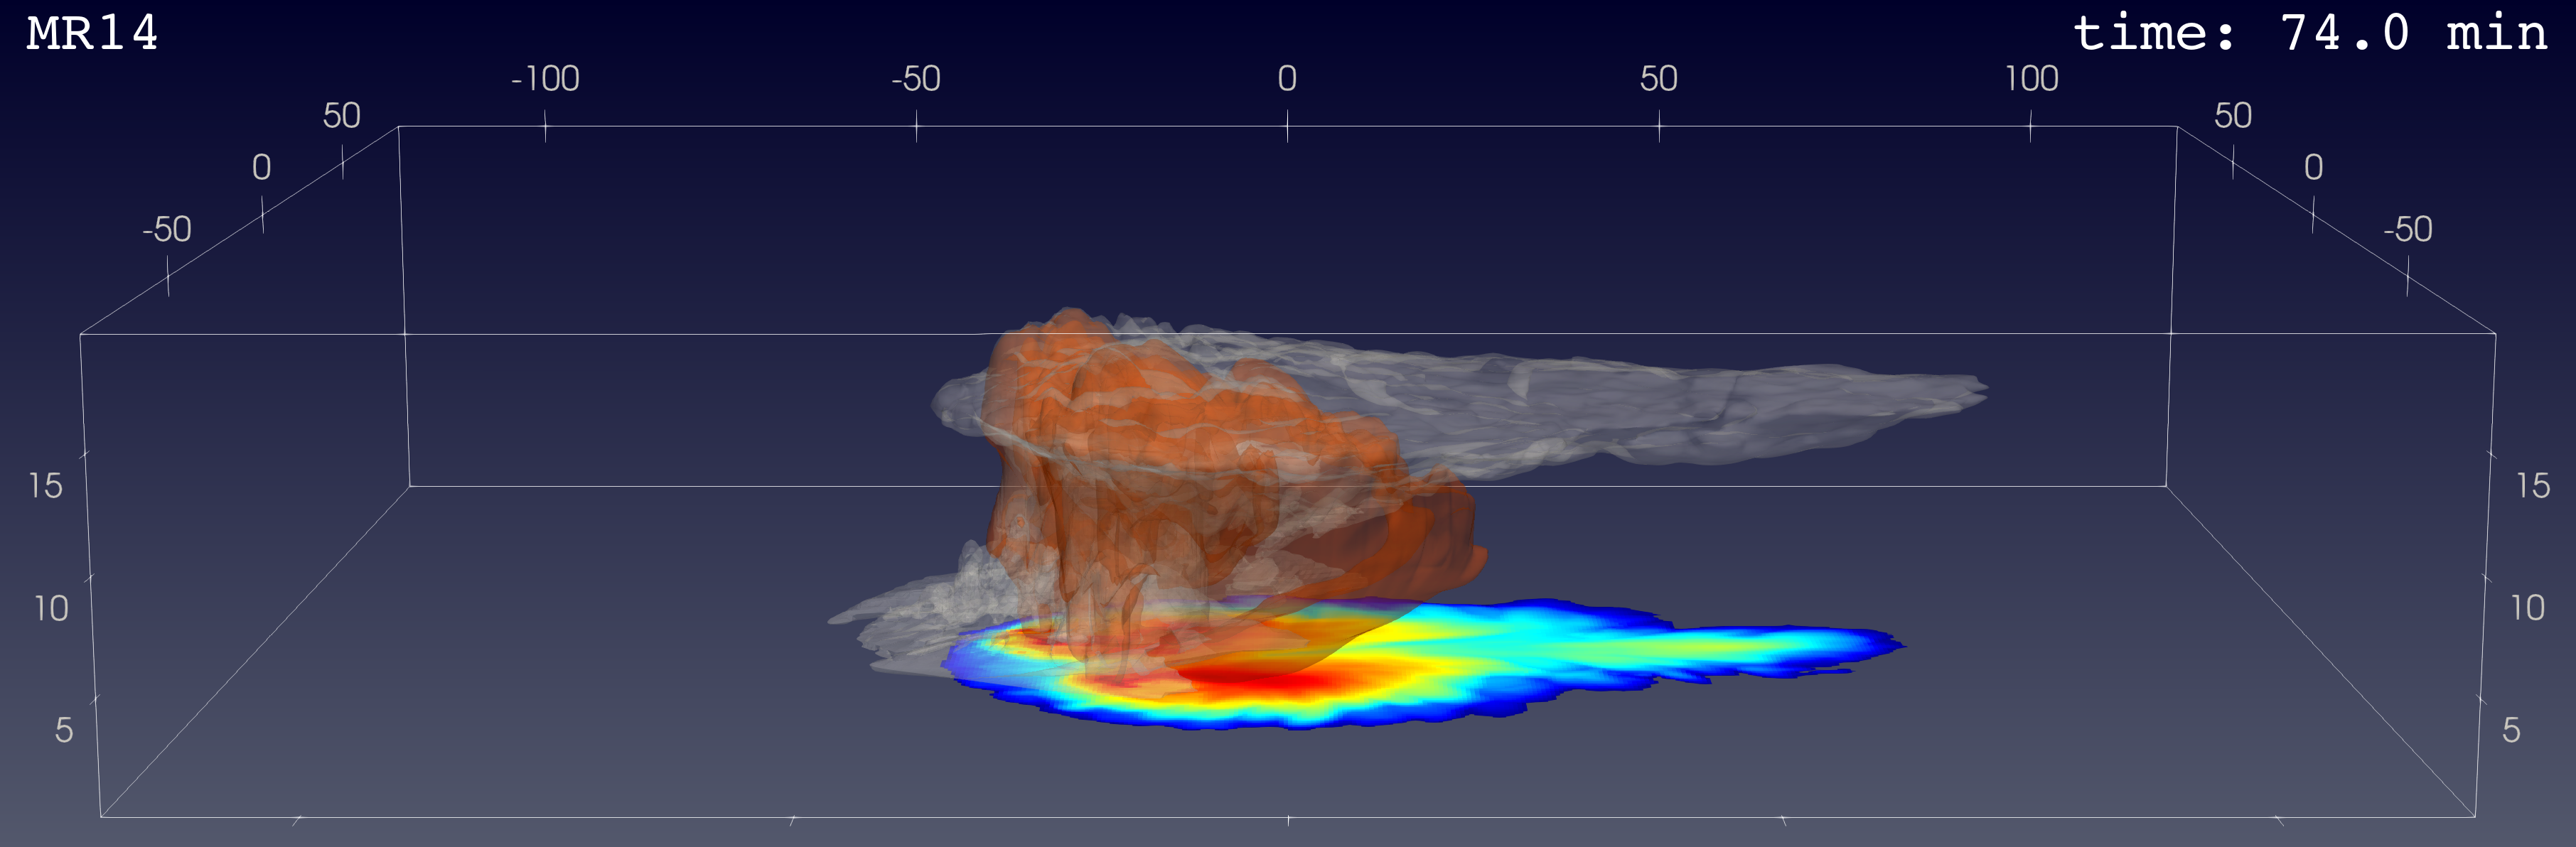
\includegraphics[width=\linewidth]{../figs/MR14-fig.0037.png}
	\caption{Die Superzelle der \texttt{MR14}-Simulation nach \SI{74}{\min} Simulationszeit. Die Konturen des Wolkenwassers sind in grau und die des Hagel-Mischungsverhältnisses in orange dargestellt. Zusätzlich ist die vertikal-integrierte maximale Reflektivität auf das niedrigste Modellniveau projiziert. Die Achsenbeschriftung gibt die Größe der Domain in \si{\km} wieder.}
	\label{fig:singleframe}
\end{figure}

In \cref{fig:cref} kann die räumliche Ausdehnung der Gewittergebilde nachvollzogen werden. In allen Simulationen ist deutlich die Aufspaltung der Superzelle in einen \textit{left-} und \textit{right-mover} zu erkennen. Dabei entstehen umso mehr lokale Gewitter entlang der Hauptpfade, je höher das Mischungsverhältnis gewählt wurde.

\begin{figure}
	\centering
	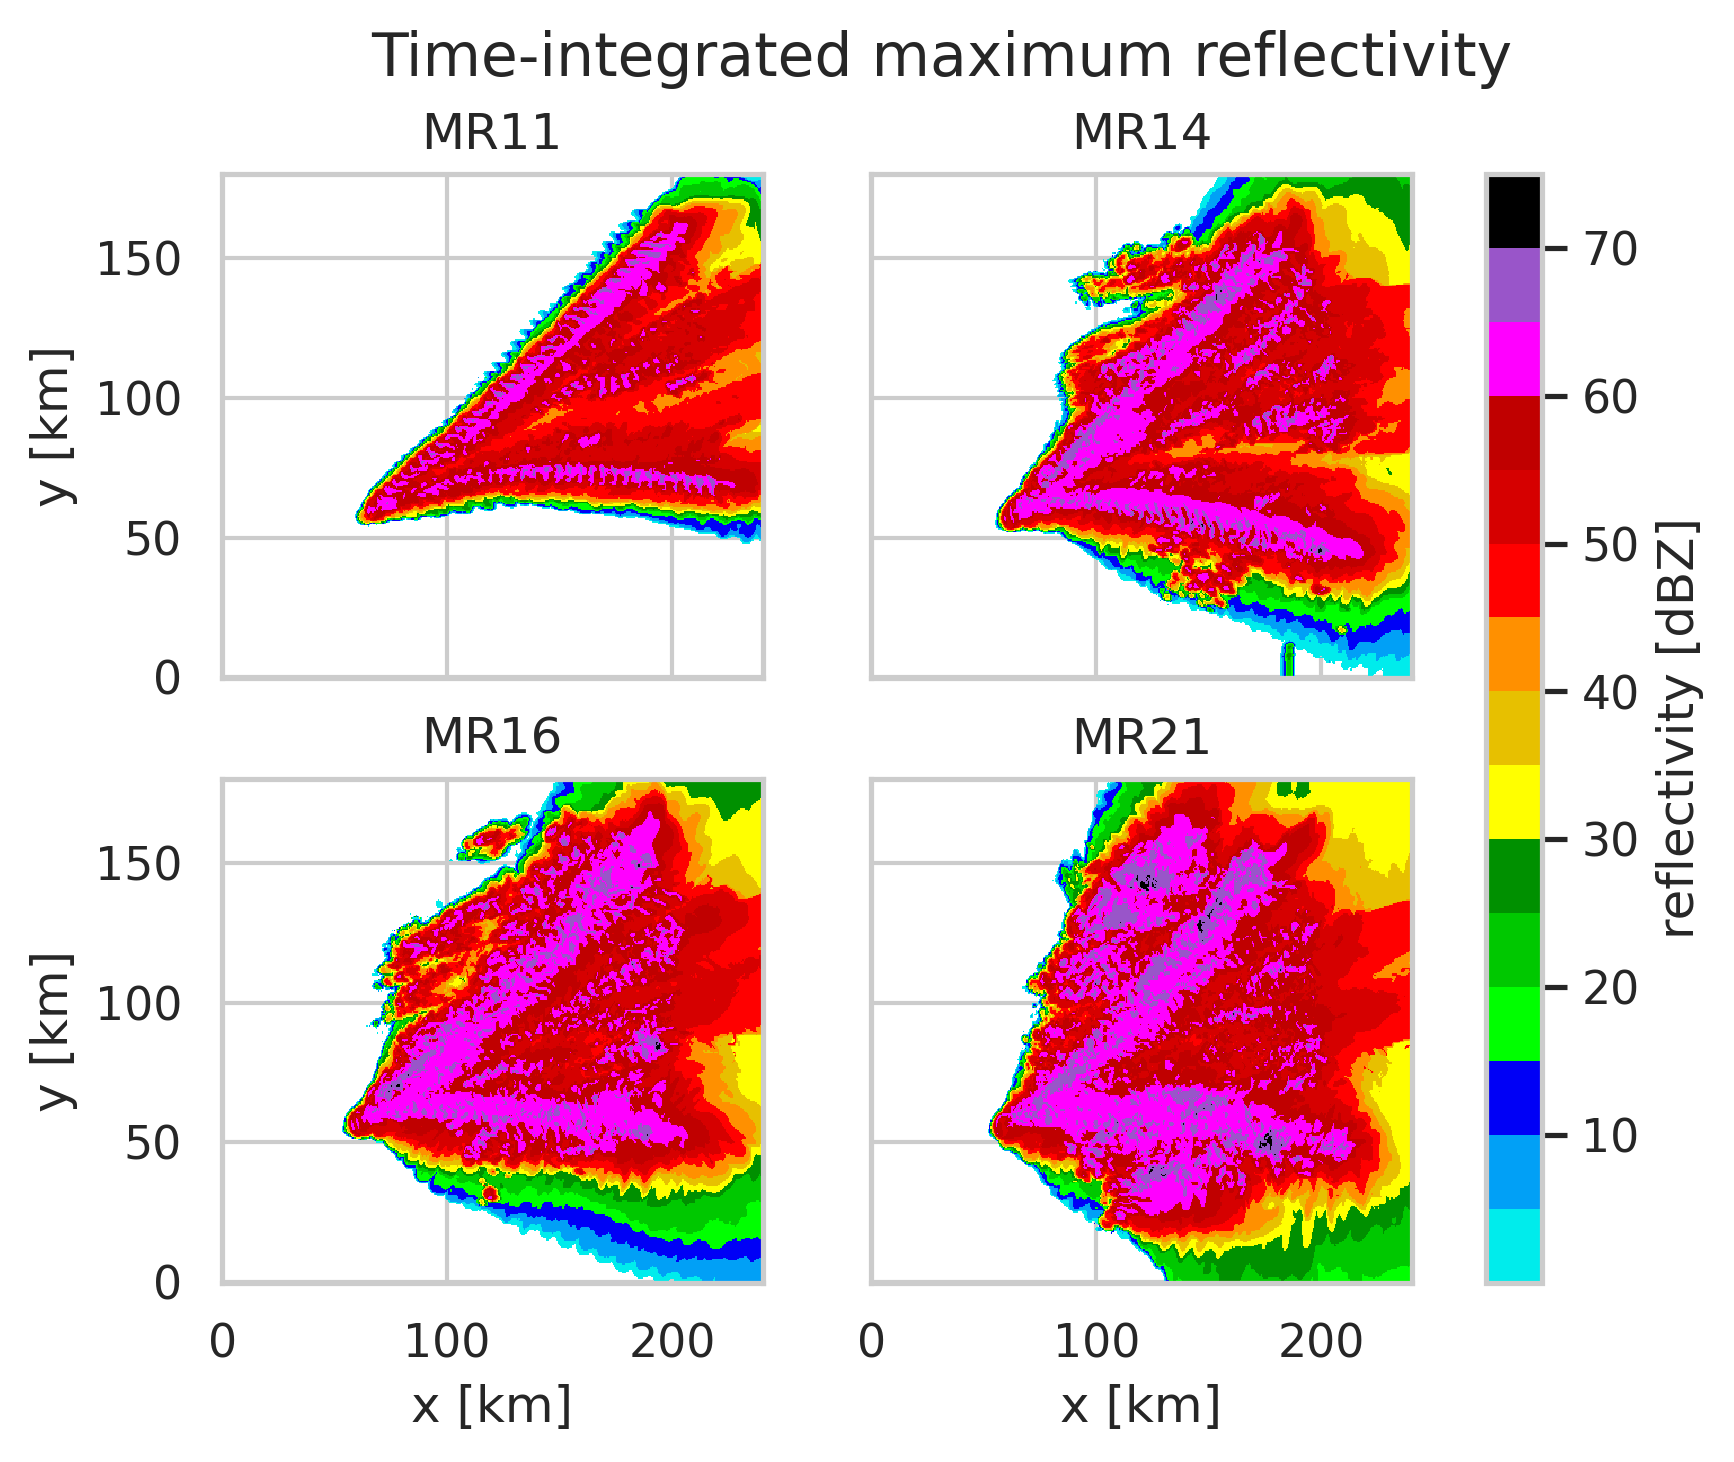
\includegraphics[width=0.8\linewidth]{../figs/cref.png}
	\caption{Die sowohl vertikal als auch zeitlich integrierte maximale Reflektivität der CM1-Simulationen}
	\label{fig:cref}
\end{figure}

Im Folgenden wird der Fokus auf die Entstehung von Hagel in den CM1-Simulationen gelegt. Daher wird der Aufwind in einer Höhe betrachtet, in der sich typischerweise Hagel bildet. Wie bereits in anderen Studien \parencite{lin2022} angenommen, wird das entsprechende Höhenintervall in dieser Analyse auf \SIrange{4}{8}{\km} AGL festgelegt. Die zeitliche Entwicklung der maximalen Vertikalgeschwindigkeit \(w\) in \cref{fig:updraft} verdeutlicht, dass eine vermehrte Verfügbarkeit von CAPE sowohl für höhere Maximalgeschwindigkeiten als auch für einen steileren Geschwindigkeitsgradienten zu Beginn der Simulation sorgt. Zur Verringerung der Maximalgeschwindigkeit bei fortgeschrittener Simulationszeit (v. a. in der \texttt{MR21}-Simulation) ist anzumerken, dass Teile des Gewittergebildes aus der Domain herauswandern. Außerdem ist der \(w \geq \SI{20}{\m\per\s}\) Aufwindbereich größer, je länger die Simulationen andauern und je höher das Mischungsverhältnis bzw. CAPE gewählt wurde.

\begin{figure}
	\centering
	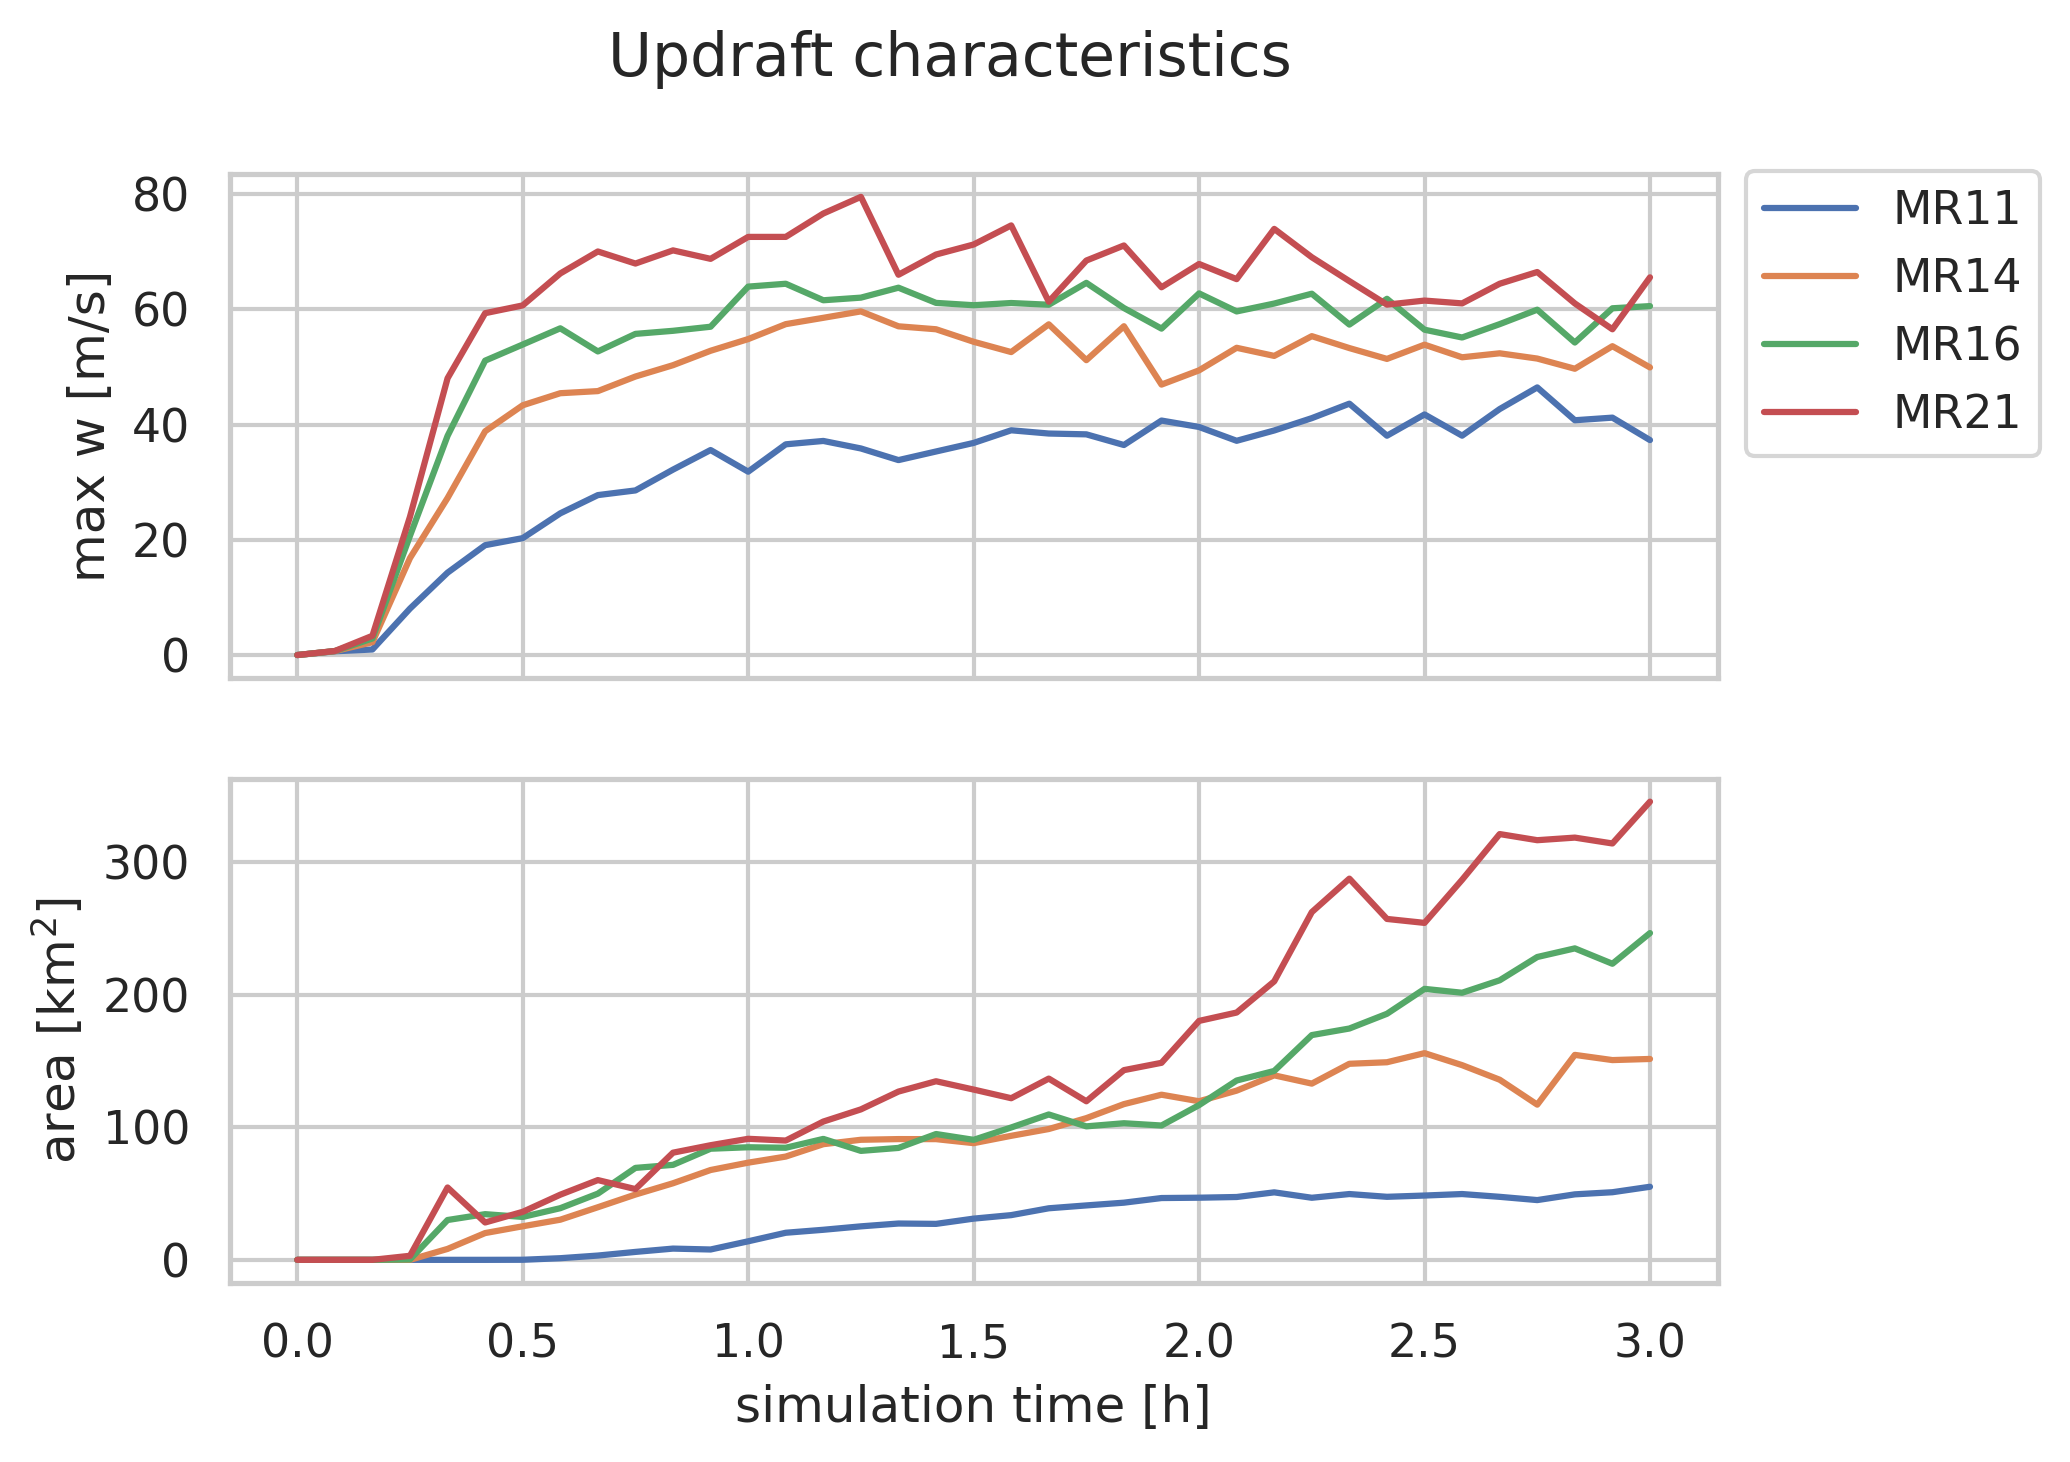
\includegraphics[width=0.9\linewidth]{../figs/updraft.png}
	\caption{\textit{Oben:} Die maximale Vertikalgeschwindigkeit des Windes über das gesamte Simulationsgebiet betrachtet. \textit{Unten:} Die gemittelte horizontale Fläche mit Aufwinden \(\geq \SI{20}{\m\per\s}\). Der Schwellenwert wurde aus \textcite{lin2022} übernommen. Beide dargestellten Größen beziehen sich auf den Bereich der optimalen Hagelentstehung zwischen \SIrange{4}{8}{\km} AGL.}
	\label{fig:updraft}
\end{figure}

Je länger die Simulationen andauern, desto mehr Hagel erreicht den Boden. Obwohl der Anstieg des Hagel-Mischungsverhältnisses \(q_h\) zunächst ähnlich zwischen den Simulationen verläuft (abgesehen von der \texttt{MR11}-Simulation, welche durchweg lediglich geringere Werte für \(q_h\) anzeigt), ändert sich dies nach ca. \SI{1.5}{\hour} Simulationszeit: Die \texttt{MR14}-Simulation erfährt eine Verringerung von \(q_h\) für etwa \SI{30}{\min}, während \texttt{MR21} ab diesem Zeitpunkt einen raschen Zuwachs an Hagel im bodennahen Bereich liefert. Darüber hinaus zeigt der rechte Subplot in \cref{fig:hail} einen Anstieg des zeitlich sowie räumlich integrierten Mittels \(\mean{q_h}\) mit zunehmendem CAPE, wobei dies für die Simulationen \texttt{MR14}-\texttt{MR21} einem linearen Zusammenhang ähnelt.

\begin{figure}
	\centering
	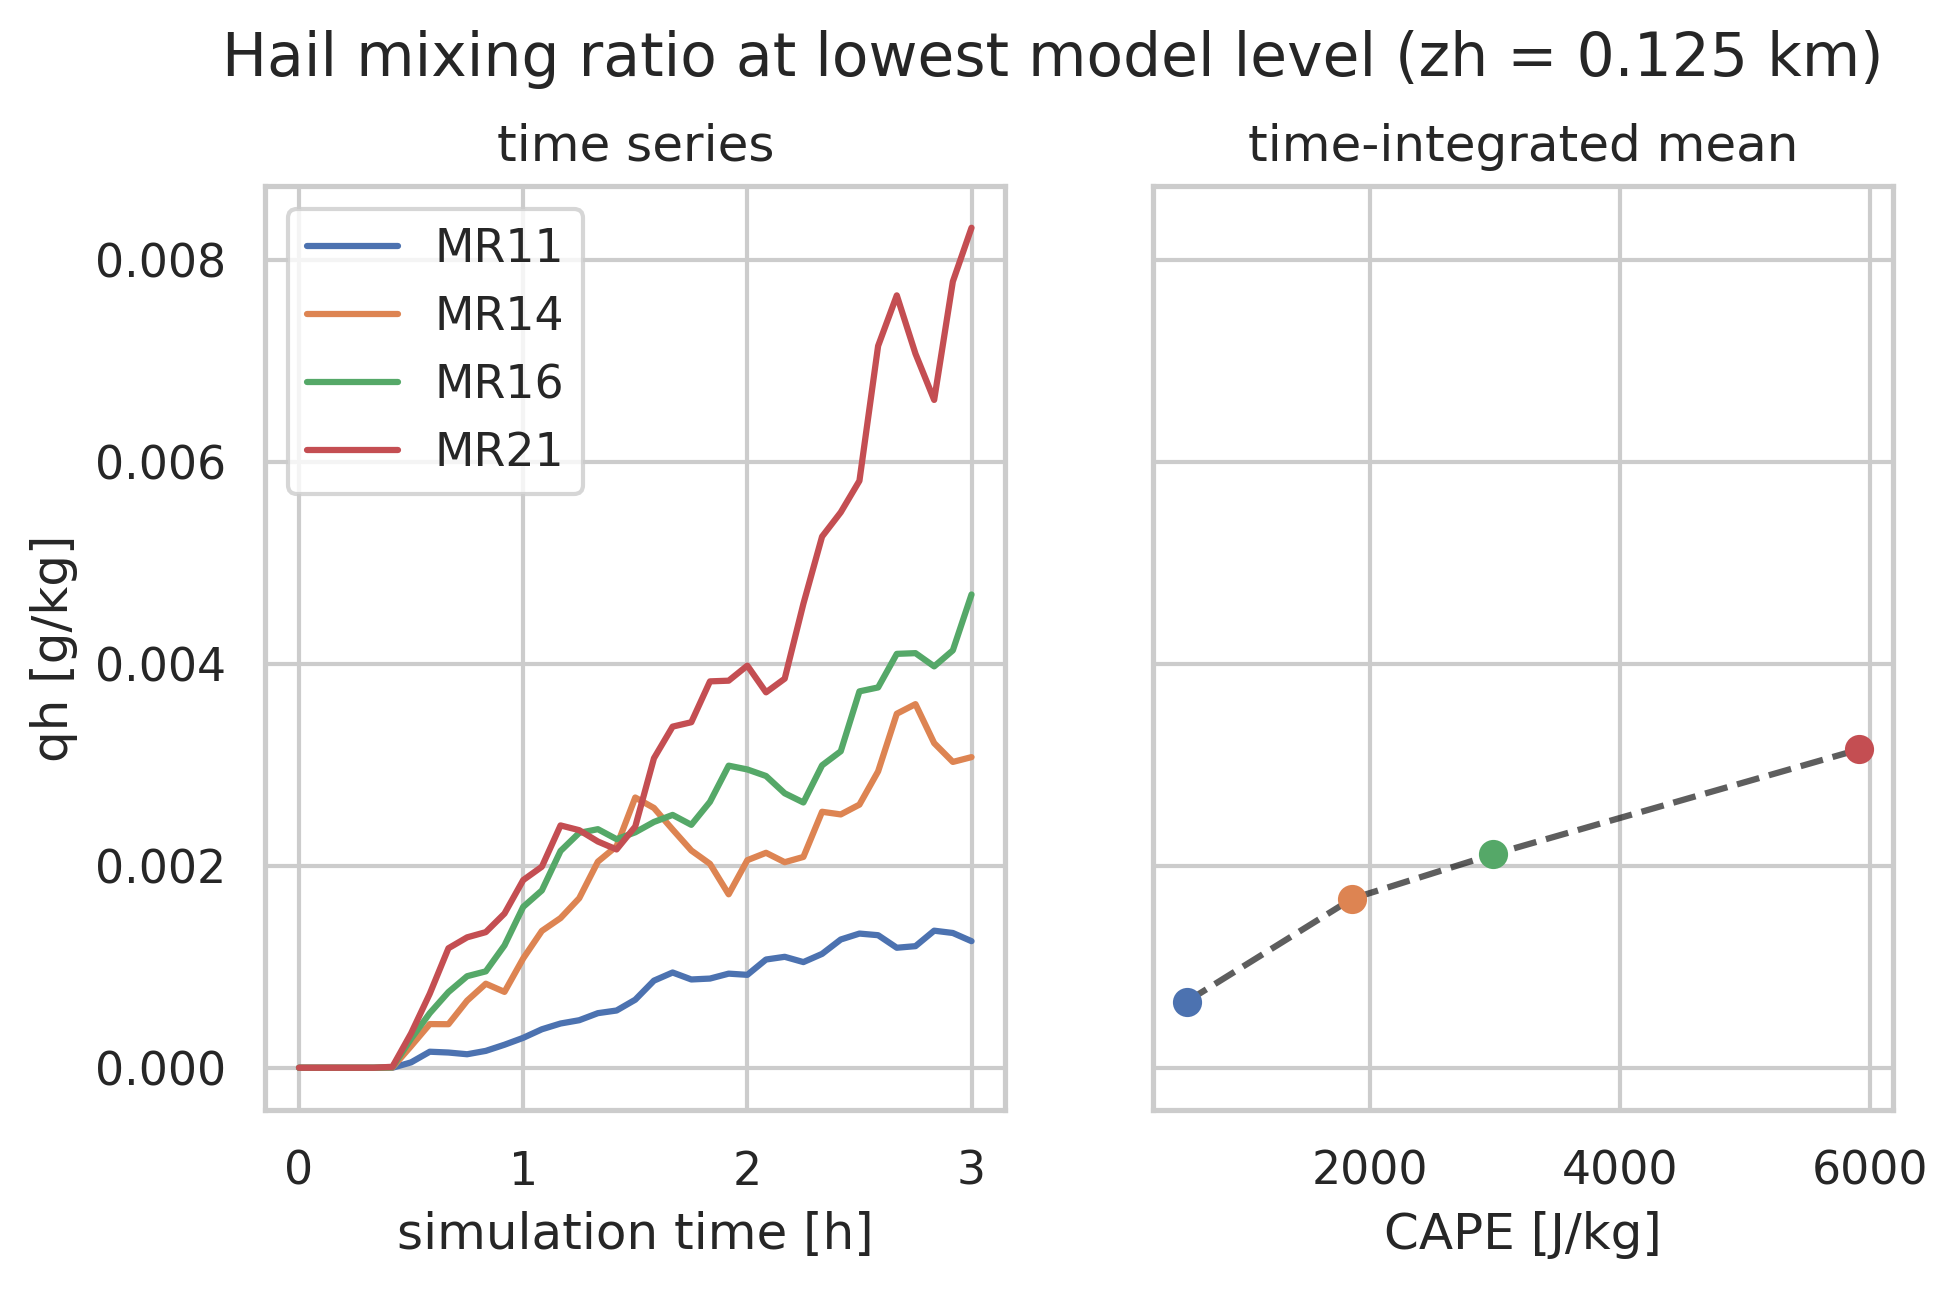
\includegraphics[width=0.9\linewidth]{../figs/hail.png}
	\caption{\textit{Links:} Die zeitliche Entwicklung des gemittelten Mischungsverhältnisses \(q_h\) von Hagel zu trockener Luft für die CM1-Simulationen. \textit{Rechts:} Das zeitliche Mittel \(\mean{q_h}\) als Funktion des CAPE. In beiden Fällen wird \(q_h\) ausschließlich auf dem niedrigsten Modellniveau berücksichtigt.}
	\label{fig:hail}
\end{figure}

Der zugrundeliegende Code dieser Analyse befindet sich auf \href{https://github.com/vegan-schnitzel/hail-supercells}{GitHub}\footnote{\hypersetup{urlcolor=}\url{https://github.com/vegan-schnitzel/hail-supercells}}. Einige der Abbildungen wurden mithilfe der python-Bibliothek \textit{MetPy} erstellt \parencite{may2016}.